\let\negmedspace\undefined
\let\negthickspace\undefined
\documentclass[journal]{IEEEtran}
\usepackage[a5paper, margin=10mm, onecolumn]{geometry}
%\usepackage{lmodern} % Ensure lmodern is loaded for pdflatex
\usepackage{tfrupee} % Include tfrupee package

\setlength{\headheight}{1cm} % Set the height of the header box
\setlength{\headsep}{0mm}     % Set the distance between the header box and the top of the text

\usepackage{gvv-book}
\usepackage{gvv}
\usepackage{cite}
\usepackage{amsmath,amssymb,amsfonts,amsthm}
\usepackage{algorithmic}
\usepackage{graphicx}
\usepackage{textcomp}
\usepackage{xcolor}
\usepackage{txfonts}
\usepackage{listings}
\usepackage{enumitem}
\usepackage{mathtools}
\usepackage{gensymb}
\usepackage{comment}
\usepackage[breaklinks=true]{hyperref}
\usepackage{tkz-euclide} 
\usepackage{listings}
% \usepackage{gvv}                                        
\def\inputGnumericTable{}                                 
\usepackage[latin1]{inputenc}                                
\usepackage{color}                                            
\usepackage{array}                                            
\usepackage{longtable}                                       
\usepackage{calc}                                             
\usepackage{multirow}                                         
\usepackage{hhline}                                           
\usepackage{ifthen}                                           
\usepackage{lscape}
\usepackage{circuitikz}


\author{EE25BTECH11041-Naman Kumar }
\graphicspath{./figs/}

\begin{document}
\begin{center}
    \huge{2.4.37}\\
    \large{EE25BTECH11041 - Naman Kumar}
\end{center}
Question:\\
Find a vector of magnitude 6, which is perpendicular to both the vectors $2\hat{\imath} - \hat{\jmath} + 2\hat{k}$ and $4\hat{\imath} - \hat{\jmath} + 3\hat{k}$\\
\solution \\
Given Vectors
\begin{align}
    \Vec{A}=\begin{pmatrix} 2\\-1\\2 \end{pmatrix}, \Vec{B}=\begin{pmatrix} 4\\-1\\3 \end{pmatrix}
\end{align}
Let required vector be,
\begin{align}
    \vec{C}=\begin{pmatrix} x\\y\\z \end{pmatrix}
\end{align}
Using Inner Product,
\begin{align}
    \vec{C}^T \cdot\vec{A}=0\text{ and }\vec{C}^T \cdot\vec{B}=0\\
    \vec{C}^T \cdot\vec{A}=2x-y+2z=0 \label{1} \\
    \vec{C}^T \cdot\vec{B}=4x-y+3z=0 \label{2}
\end{align}
Using Rank to Analyze the system
\begin{align}
    2x-y+2z,4x-y+3z\\
    \vec{A}=\begin{pmatrix} 2&-1&2\\4&-1&3 \end{pmatrix}
\end{align}
Using Row Transformations to Get Row Reduced echelon Form
\begin{align}
    \vec{A}=\begin{pmatrix} 2&-1&2\\4&-1&3 \end{pmatrix} \xrightarrow[]{R_2 \rightarrow R_2-2R_1}\begin{pmatrix} 2&-1&2\\0&1&-1 \end{pmatrix}\\
    \xrightarrow[]{R_1 \rightarrow \frac{1}{2}R_1}\begin{pmatrix} 1&\frac{-1}{2}&1\\0&1&-1 \end{pmatrix}\\
    \xrightarrow[]{R_1 \rightarrow R_1+\frac{1}{2}R_2}\begin{pmatrix} 1&0&\frac{1}{2}\\0&1&-1 \end{pmatrix}\\
    \vec{A}=(\vec{I}\vec{X}), \text{\textbf{I} is identity matrix}
\end{align}
And, $\vec{X}$ is
\begin{align}
    \begin{pmatrix}\frac{1}{2}\\-1\end{pmatrix}
\end{align}
Since rank of matrix is 2($\leq 3$), their are infinite many solutions $R^3\rightarrow R^2$\\
From the Row Reduced Echelon form(RREF),we can write the new system of equation:
\begin{align}
    x+\frac{1}{2}z=0 \label{3} \\
    y-z=0 \label{4}
\end{align}
Therefore vector $\vec{C}$ using equations $\eqref{3}$ and $\eqref{4}$ is
\begin{align}
    \vec{C}=\begin{pmatrix}x\\-2x\\-2x\end{pmatrix}=x\begin{pmatrix}1\\-2\\-2\end{pmatrix}
\end{align}
Now getting vector with magnitude 6
\begin{align}
    \lVert C\rVert =6\\
    \lVert x\rVert \sqrt{(1)^2+(-2)^2+(-2)^2}=6\\
    \lVert x\rVert \sqrt{1+4+4}=6\\
    \lVert x\rVert \sqrt{9}=6\\
    \lVert x\rVert =2
\end{align}
Therefore final vectors are
\begin{align}
    C_1=\begin{pmatrix} -2\\4\\4 \end{pmatrix},
    C_2=\begin{pmatrix} 2\\-4\\-4 \end{pmatrix}
\end{align}
\begin{figure}[H]
    \centering
    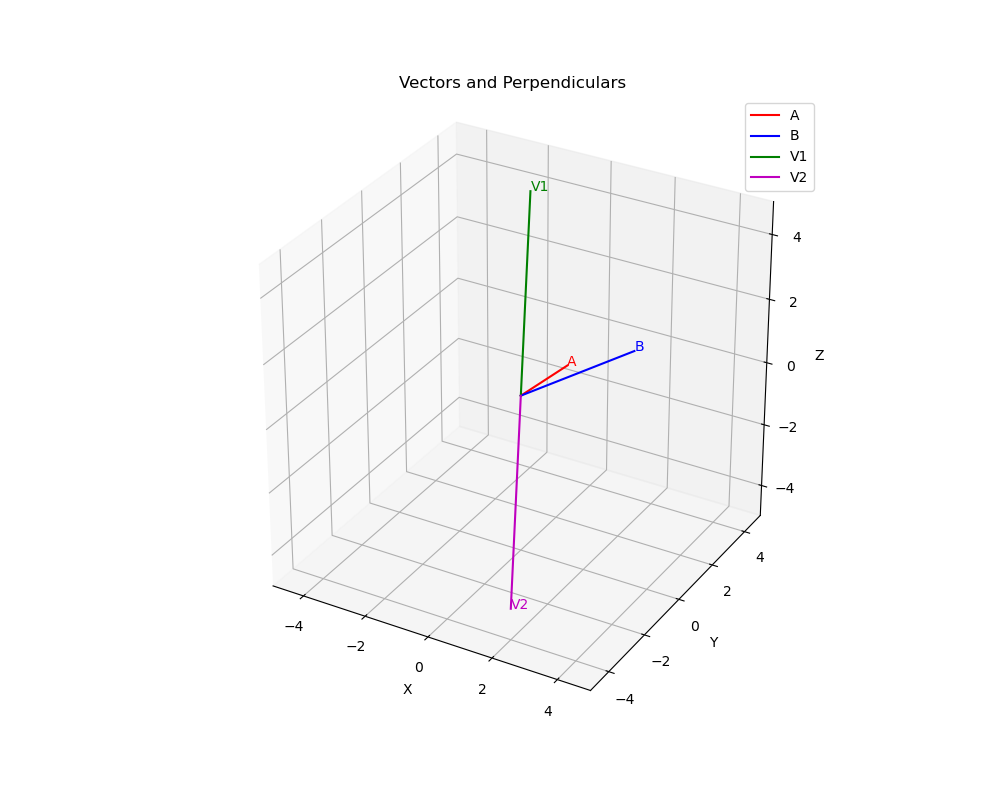
\includegraphics[width=\columnwidth]{figs/vector_plot.png}
    \caption{}
    \label{fig:placeholder}
\end{figure}
\end{document}
